\documentclass[11pt]{article}
\usepackage[T1]{fontenc}
\usepackage[utf8]{inputenc}
\usepackage{lmodern}
\usepackage[margin=1in]{geometry}
\usepackage{amsmath,amssymb,amsthm,mathtools}
\usepackage{enumitem}
\usepackage{microtype}
\usepackage{xcolor}
\usepackage{tikz}
\usepackage[nottoc,notlof,notlot,notindex]{tocbibind}
\usepackage[unicode,colorlinks=true,linkcolor=blue!45!black,citecolor=blue!45!black,urlcolor=blue!45!black]{hyperref}
\numberwithin{equation}{section}
\newtheorem{theorem}{Theorem}[section]
\newtheorem{lemma}[theorem]{Lemma}
\newtheorem{proposition}[theorem]{Proposition}
\newtheorem{corollary}[theorem]{Corollary}
\theoremstyle{definition}
\newtheorem{definition}[theorem]{Definition}
\theoremstyle{remark}
\newtheorem{remark}[theorem]{Remark}
\newcommand{\R}{\mathbb R}
\newcommand{\N}{\mathbb N}
\newcommand{\E}{\mathbb E}
\renewcommand{\P}{\mathbb P}
\newcommand{\1}{\mathbf 1}
\newcommand{\FUSF}{\mathrm{FUSF}}
\newcommand{\WUSF}{\mathrm{WUSF}}
\newcommand{\norm}[1]{\left\lVert#1\right\rVert}
\newcommand{\abs}[1]{\left|#1\right|}
\DeclareMathOperator{\Cov}{Cov}
\DeclareMathOperator{\Var}{Var}
\setlist{itemsep=3pt,topsep=5pt}
\setlength{\emergencystretch}{1em}
\title{The free uniform spanning forest is a factor of IID}
\author{OpenAI}
\date{September 25, 2026}
\hypersetup{pdftitle={The free uniform spanning forest is a factor of IID},pdfauthor={OpenAI}}
\begin{document}
\maketitle
\begin{abstract}
We prove that the free uniform spanning forest is a factor of IID on every
infinite connected locally finite simple unweighted graph. One Borel rule works
for all such graphs and uses no root, answering affirmatively the general factor
question for unimodular random graphs. We also show that every
translation-invariant strongly Rayleigh process indexed by a
countable group is a factor of IID, including invariant determinantal
processes with Hermitian positive-contraction kernels. This group-action
conclusion requires no amenability.
\end{abstract}
\section{Introduction}
\label{sec:introduction}

Uniform spanning forests are canonical probability measures on the edges of
an infinite graph. Pemantle constructed infinite-volume spanning-tree limits
on the integer lattice~\cite[Theorem~2.3]{Pemantle1991}; Benjamini, Lyons,
Peres and Schramm developed their general graph theory~\cite{BLPS2001}. The free uniform spanning forest is obtained by taking
weak limits of uniform spanning trees on finite connected exhaustions, without
identifying boundary vertices. The limit exists and is independent of the
exhaustion. We recall its classical construction from finite tree determinants
in Proposition~\ref{prop:free-limit}; see also Benjamini, Lyons, Peres, and
Schramm~\cite[Section~5]{BLPS2001}.
A factor of IID description asks whether this global random object can be
constructed, equivariantly and measurably, from independent labels attached
to the vertices. Lyons explicitly discussed the FUSF factor question for
the group action on Cayley graphs in his report for the 2013 Oberwolfach
workshop~\cite[p.~2392]{Lyons2013}.

On transient graphs, the wired forest has an IID construction through
cycle popping and Wilson's algorithm rooted at infinity; see
\cite[Theorem~5.1]{BLPS2001}. Angel, Ray and Spinka give an explicit
graph-factor formulation, retaining the transient graph scope and crediting
the earlier construction~\cite[Section~4]{AngelRaySpinka2024}. Determinantal structure also provides
factor constructions in amenable group settings: Lyons and Thom prove
Bernoulli isomorphism for equivariant determinantal measures on amenable
Cayley graphs, with respect to the group action \cite[Corollary~7.4]{LyonsThom2016}. This Bernoulli-isomorphism result concerns
the specified group action; it does not by itself provide one rule
on arbitrary graphs equivariant under every graph isomorphism.

For general graph laws, Tim\'ar proves FIID representability of the free
forest on recurrent unimodular random graphs and, more generally, on
invariantly amenable unimodular random graphs
\cite[arXiv version, Theorem~1 and Corollary~5]{Timar2025}.
Under invariant amenability he obtains the stronger conclusion of a
finite-valued finitary factor~\cite[arXiv version, Theorem~2(1)]{Timar2025}.
His construction uses compatible monotone finite-volume limits along a
hyperfinite exhaustion. The introduction to that December 2025 version
states the unrestricted FUSF factor question as open. We prove the
unrestricted graphwise statement by a different construction: the same
Borel rule works for every graph in our class, independently of any
random-graph law. The challenge is to obtain a single equivariant sample
from the infinite-volume law while controlling all edges jointly.

\subsection{Statement}

The graphs in our main result are infinite, connected, locally finite, simple,
and undirected. Write $\FUSF_G$ for the free uniform spanning forest law on
$\{0,1\}^{E(G)}$. Graphs with a distinguished undirected edge and vertex
labels carry the usual Borel structure generated by finite marked
neighborhoods. A rule is \emph{root independent} if it uses no distinguished
vertex. Equivariance means invariance under every isomorphism of labeled
graphs carrying the distinguished edge to the distinguished edge.

\begin{theorem}\label{thm:main}
There is one Borel, root-independent, equivariant rule
\[
 \Phi(G,U,e)\in\{0,1\}
\]
such that, for every infinite connected locally finite simple undirected
unweighted graph $G$ and independent
$\operatorname{Uniform}[0,1]$ vertex labels $U=(U_v)_{v\in V(G)}$, the entire
edge set
\[
 \{e\in E(G):\Phi(G,U,e)=1\}
\]
has law $\FUSF_G$.
\end{theorem}

\begin{corollary}\label{cor:unimodular}
The free uniform spanning forest is a graph factor of IID under every
unimodular law supported on the stated class of graphs. The same rule works
for every such law.
\end{corollary}

Here unimodularity means the mass-transport identity
\[
 \E\sum_{v\in V(G)} f(G,o,v)
 =\E\sum_{v\in V(G)} f(G,v,o)
\]
for every nonnegative Borel function of a graph with two distinguished
vertices. Theorem~\ref{thm:main} is a graphwise statement and does not use
this identity. In particular, no amenability, transience, uniform degree
bound, or degree moment is assumed. The result asserts an ordinary Borel
factor, without a finitary coding radius or a finite input alphabet.

\subsection{Strongly Rayleigh processes}

The sampling criterion also applies to a broader class of binary laws.
For a finite set $F$, a probability measure $\mu$ on $\{0,1\}^F$ is
\emph{strongly Rayleigh} if its generating polynomial
\[
 g_\mu(z)=\sum_{x\in\{0,1\}^F}\mu(x)\prod_{i\in F}z_i^{x_i}
\]
is nonzero whenever $\operatorname{Im}z_i>0$ for every $i\in F$.
For a countable index set, we require every finite-coordinate marginal to
be strongly Rayleigh, following Borcea, Br\"and\'en, and
Liggett~\cite[Definition~2.13]{BorceaBrandenLiggett2009}.

For a countable group $\Gamma$, write $\tau_g$ for the regular left action
on coordinate families, given by $(\tau_g a)_h=a_{g^{-1}h}$.

\begin{theorem}[Strongly Rayleigh processes on countable groups]
\label{thm:sr-group}
Let $\Gamma$ be a countable group and let $\nu$ be a strongly Rayleigh
probability law on $\{0,1\}^{\Gamma}$ invariant under every $\tau_g$.
There is a Borel map
\[
 \Phi_\nu:[0,1]^{\Gamma}\longrightarrow\{0,1\}^{\Gamma}
\]
such that $\Phi_\nu(\tau_g u)=\tau_g\Phi_\nu(u)$ for every $g\in\Gamma$
and every $u\in[0,1]^{\Gamma}$, and such that $\Phi_\nu(U)$ has law $\nu$
when the coordinates of $U$ are independent $\operatorname{Uniform}[0,1]$
variables.
\end{theorem}

For a self-adjoint positive contraction $K$ on $\ell^2(\Gamma)$, the
determinantal law of a random subset $X\subseteq\Gamma$ is characterized
by the finite inclusion probabilities
\[
 \P(A\subseteq X)=\det(K_{g,h})_{g,h\in A}
 \qquad\text{for every finite }A\subseteq\Gamma.
\]

\begin{corollary}[Determinantal processes on countable groups]
\label{cor:dpp-group}
Let $\Gamma$ be a countable group and let $K$ be a self-adjoint positive
contraction on $\ell^2(\Gamma)$, so $0\le K\le I$. If the determinantal
probability law with kernel $K$ is invariant under the regular left action,
then it is a factor of IID under that action. In particular, this holds
whenever $K$ commutes with the left regular representation of $\Gamma$.
\end{corollary}

These statements concern the regular action on the group itself, not an
arbitrary action on another index set. The factor may depend on $\Gamma$
and $\nu$. No amenability or finite-generation assumption is imposed, and
finite groups are allowed. The conclusion is a Borel factor of IID; it
does not assert a finitary coding or a Bernoulli isomorphism. In particular,
it is distinct from the amenable-group Bernoulli-isomorphism result of
Lyons and Thom cited above. Their broader determinantal factor question
appears in~\cite[Question~7.7]{LyonsThom2016}; Corollary~\ref{cor:dpp-group}
treats the regular action on the group itself.

\subsection{The construction}

Let $X$ have the target forest law and observe its edge indicators through
independent Brownian noises:
\[
 Y_e(t)=tX_e+B_e(t).
\]
For finitely many observed edges, the posterior is an exponential tilt of
the forest law. The main quantitative input is the following response
identity for a finite weighted spanning tree. If $p_e$ is the probability
of including edge $e$ and $h_f$ is the logarithm of the weight of edge $f$,
then
\[
 \sum_f\left|\frac{\partial p_e}{\partial h_f}\right|
 =2p_e(1-p_e)\le\frac12.
\]
Negative off-diagonal covariances and the fixed size of a finite tree give
this identity. Passing it through finite-volume limits yields an
everywhere-defined posterior drift $b(t,y)$ whose response to bounded
changes of the field is uniformly Lipschitz, even when the fields themselves
are unbounded across the graph.

Subtracting the posterior drift gives the innovations
\[
 \widehat W_e(t)=Y_e(t)-\int_0^t b_e(s,Y(s))\,ds.
\]
They are independent Brownian motions. The response bound makes the integral
equation
\[
 Z_e(t)=w_e(t)+\int_0^t b_e(s,Z(s))\,ds
\]
uniquely solvable by a Borel Picard iteration for every continuous input
field $w$. Only differences between iterates are bounded; there is no
assumption that a countable Brownian field takes values in $\ell^\infty$.
Thus $Y=Z(\widehat W)$, and independent Brownian inputs to this deterministic
decoder reproduce the observation law. Integer-time slopes recover $X$.

Proposition~\ref{prop:brownian-sampler} isolates the resulting sampling
criterion for countable binary laws with uniformly controlled finite-tilt
responses. The criterion separates the probabilistic observation argument
from the quantitative property of the target measure. For spanning forests,
intrinsic edge-centered balls make the decoder equivariant across graphs.
Finally, independent vertex labels supply the independent edge paths by a
local allocation of disjoint random coordinates.

This construction adapts an established observation mechanism. Stochastic
localization was introduced by Eldan~\cite{Eldan2013}; a finite-dimensional
form with fixed noise covariance appears
in~\cite[Section~2, Proposition~7]{Eldan2020}. El Alaoui and
Montanari~\cite[Section~3, Theorem~2]{ElAlaouiMontanari2022} develop its
Gaussian-channel observation and innovation formulation. A particularly
close antecedent is Nam, Sly and
Zhang~\cite[Theorem~1 and Section~2.2]{NamSlyZhang2022}: for free Ising
measures on regular trees in their parameter range, they obtain FIID
codings through Brownian-driven systems with posterior-mean drift and
recover spins at large times. Here we prove the countable-coordinate
posterior and joint innovation identities, then use the uniform response
bound to obtain an inverse defined at every continuous input.

A companion~\cite[Theorem~1.1]{SharpFreeIsing2026} gives the sharp FIID
threshold for the free zero-field ferromagnetic Ising law on regular
trees, including the critical case, with a factor that can be chosen to commute
with every tree automorphism on every label input. Its conditional-copy recovery
differs from our uniform-response inverse.

For strongly Rayleigh laws, symmetric homogenization supplies a fixed-size
strongly Rayleigh extension, and the Rayleigh inequality gives nonpositive
off-diagonal covariances~\cite[Definition~2.12 and Theorems~4.1--4.2]{BorceaBrandenLiggett2009}.
The covariance-row bound then holds with the same constant $1/2$, as an
inequality rather than the weighted-tree identity. Translates of one finite
exhaustion of $\Gamma$ make the resulting drift equivariant for the regular
group action.

Section~\ref{sec:response} reconstructs the free limit and establishes the
response estimate and the canonical
drift. Section~\ref{sec:observation} proves the posterior and innovation
identities. The deterministic inverse and sampling criterion follow in
Section~\ref{sec:decoder}. Section~\ref{sec:implementation} constructs the
single Borel graph rule and proves Theorem~\ref{thm:main}.
Section~\ref{sec:strongly-rayleigh} proves Theorem~\ref{thm:sr-group} and
Corollary~\ref{cor:dpp-group}.

\section{Weighted trees and a canonical response field}
\label{sec:response}

The analytic input is a response estimate whose constant is independent
of the number of edges and of their weights.  We first prove it on finite
graphs, then use the free spanning-tree limit to construct a
drift on every field of real edge marks. The finite determinant and
transfer-current identities are classical; see Burton and
Pemantle~\cite{BurtonPemantle1993} and the weighted formulation in
\cite[Section~4]{BLPS2001}. We prove the needed identities and their
free-limit consequence below.

\begin{lemma}[Weighted-tree response]
\label{lem:tree-response}
Let $H$ be a finite connected graph with at least two vertices, and let
$\mathcal T(H)$ denote its set of spanning trees.  For
$h\in\mathbb R^{E(H)}$, give each $T\in\mathcal T(H)$ probability
proportional to $\exp(\sum_{f\in T}h_f)$, and write
$\xi_e=\1_{\{e\in T\}}$ and $p_e(h)=\mathbb E_h\xi_e$.
For every $e\in E(H)$,
\begin{equation}
\label{eq:covariance-row}
\frac{\partial p_e}{\partial h_f}
 =\operatorname{Cov}_h(\xi_e,\xi_f),
\qquad
\sum_{f\in E(H)}
 \left|\frac{\partial p_e}{\partial h_f}\right|
 =2p_e(h)(1-p_e(h))\le\frac12.
\end{equation}
In particular, for all $h,h'\in\mathbb R^{E(H)}$,
\begin{equation}
\label{eq:tree-response}
 |p_e(h)-p_e(h')|
 \le\frac12\max_{f\in E(H)}|h_f-h'_f|.
\end{equation}
\end{lemma}

\begin{proof}
Set $c_f=e^{h_f}$.  Orient the edges temporarily, delete one row of the
oriented incidence matrix, and denote the resulting columns by $a_f$.
The reduced weighted Laplacian is
\[
 L=\sum_{f\in E(H)}c_fa_fa_f^{\mathsf T}.
\]
Write $r=|V(H)|-1$.  Cauchy--Binet, applied to the reduced incidence
matrix with column $f$ multiplied by $\sqrt{c_f}$, gives
\[
 \det L
 =\sum_{\substack{F\subseteq E(H)\\|F|=r}}
   \det(a_f:f\in F)^2\prod_{f\in F}c_f
 =\sum_{T\in\mathcal T(H)}\prod_{f\in T}c_f
 =:\mathcal Z_H(h).
\]
For the second equality, a set containing a cycle has dependent
incidence columns, while an acyclic set of $r$ edges is a spanning
tree.  Its reduced incidence determinant has absolute value one:
expand at a leaf other than the vertex whose row was deleted and
continue by induction.  Connectedness supplies a spanning tree, so
$\mathcal Z_H(h)>0$ and $L$ is invertible.

Differentiating the finite partition sum gives both
$p_e=\partial_{h_e}\log\mathcal Z_H$ and the covariance identity in
\eqref{eq:covariance-row}.  Differentiating the determinant instead gives
\[
 p_e=c_ea_e^{\mathsf T}L^{-1}a_e.
\]
Since
$\partial_{h_f}L^{-1}=-c_fL^{-1}a_fa_f^{\mathsf T}L^{-1}$,
for distinct edges $e,f$ we obtain
\begin{equation}
\label{eq:negative-square}
 \operatorname{Cov}_h(\xi_e,\xi_f)
 =-c_ec_f\bigl(a_e^{\mathsf T}L^{-1}a_f\bigr)^2\le0.
\end{equation}
Every spanning tree has exactly $r$ edges.  Consequently
\[
 \sum_{f\in E(H)}\operatorname{Cov}_h(\xi_e,\xi_f)
 =\operatorname{Cov}_h\!\left(\xi_e,
                  \sum_{f\in E(H)}\xi_f\right)=0.
\]
The diagonal covariance is $p_e(1-p_e)$; all the other covariances
are nonpositive by \eqref{eq:negative-square}.  Their absolute sum
is therefore $2p_e(1-p_e)\le1/2$, as claimed.  This also covers a
bridge: its inclusion probability is one and its entire covariance
row is zero.  Finally, integrate the gradient along the segment from
$h$ to $h'$ to obtain \eqref{eq:tree-response}.  The estimate holds
at every point of that segment, without a restriction on the weights.
\end{proof}

\subsection{The free limit from finite determinants}

We include the free-limit construction, so that the passage from finite
weighted trees to the infinite law has an explicit foundation. The relevant
space is the closure of the finite cycle flows; no description of all
square-summable divergence-free flows on the infinite graph is needed.
This cycle-space description is classical; see
\cite[Proposition~7.1 and Theorem~7.8]{BLPS2001}.

\begin{proposition}[Free exhaustion limit]\label{prop:free-limit}
Let $G$ be an infinite connected locally finite simple graph. If
$H_1\subseteq H_2\subseteq\cdots$ are finite connected subgraphs with
$\bigcup_n E(H_n)=E(G)$, the uniform spanning-tree laws on $H_n$, extended
by absent edges outside $H_n$, converge weakly on $\{0,1\}^{E(G)}$.
Their limit is independent of the exhaustion, is supported on spanning
forests, and is transported by every graph isomorphism. We denote this
law by $\FUSF_G$.
\end{proposition}

\begin{proof}
Temporarily orient all edges of $G$. For a finite connected subgraph $H$
with at least two vertices, let $A_H$ be its reduced incidence matrix and
put
\[
 K_H=A_H^{\mathsf T}(A_HA_H^{\mathsf T})^{-1}A_H.
\]
For each finite $F\subseteq E(H)$, the matrix-tree calculation in
Lemma~\ref{lem:tree-response}, followed by the rectangular determinant
identity, gives the polynomial identity
\begin{align}
 \E\prod_{e\in F}(1+z_e\xi_e)
 &=\frac{\det(A_HA_H^{\mathsf T}
        +A_F\operatorname{diag}(z)A_F^{\mathsf T})}
        {\det(A_HA_H^{\mathsf T})} \notag\\
 &=\det\!\left(I_F+\operatorname{diag}(z)(K_H)_{F,F}\right).
 \label{eq:finite-inclusion-polynomial}
\end{align}
Here $A_F$ consists of the columns indexed by $F$. The first equality
can first be read for $z_e>-1$ as a change of edge weights, and then
holds for all $z$ because both sides are polynomials. The identity
$\det(I+UV)=\det(I+VU)$ used in the second line follows by eliminating
blocks in $\left(\begin{smallmatrix}I&U\\-V&I\end{smallmatrix}\right)$
in either order. Expanding the last determinant in its diagonal variables
and comparing coefficients yields
\begin{equation}\label{eq:finite-inclusion-minor}
 \P(F\subseteq T_H)=\det (K_H)_{F,F}.
\end{equation}
This includes sets larger than $|V(H)|-1$: the corresponding minor and
tree-inclusion probability are both zero. No minor is inverted.

Regard finite edge vectors as vectors of $\ell^2(E(G))$ by zero extension.
Let $C_H=\ker A_H$ in the coordinates of $E(H)$, and let $Q_H$ be the
orthogonal projection onto those coordinates. The matrix $K_H$ is the
orthogonal projection onto the row space of $A_H$, so its zero extension is
\begin{equation}\label{eq:finite-cycle-projection}
 K_H=Q_H-P_{C_H}.
\end{equation}
Deleting a different incidence row does not change $C_H$: the full
incidence matrix has entries summing to zero in each column, so zero
divergence at all but one vertex
forces zero divergence at the remaining vertex. The space $C_H$ is exactly
the span of its oriented cycle flows. Indeed, choose a spanning tree of
$H$ and subtract the fundamental cycle flow for each non-tree edge to
eliminate that edge's coefficient. The remaining circulation is supported
on a tree and vanishes by successive leaf removal.

Write $C_n=C_{H_n}$. These spaces increase under zero extension: a
circulation supported on $H_n$ still has zero divergence at every vertex
of $H_{n+1}$. Every finite cycle of $G$ is eventually contained in $H_n$,
because the exhaustion includes every edge. Therefore the closure
\[
 C=\overline{\bigcup_n C_n}
\]
is the closed span of all finite cycle flows of $G$, independent of the
chosen exhaustion, whether or not its members are induced subgraphs.
The projections $P_{C_n}$ converge strongly to $P_C$. To see this directly,
for $m\ge n$ and $x\in\ell^2(E(G))$ orthogonality gives
\[
 \|P_{C_m}x-P_{C_n}x\|^2
 =\|P_{C_m}x\|^2-\|P_{C_n}x\|^2.
\]
The squared norms increase and are bounded by $\|x\|^2$, so the projected
vectors are Cauchy. Their limit lies in $C$, and its difference from $x$
is orthogonal to every $C_n$, hence to $C$. This identifies the limit as
$P_Cx$. Also $Q_{H_n}\to I$ strongly. Thus the zero-extended $K_{H_n}$
converge strongly to $K=I-P_C$, and every fixed finite principal minor
converges to that of $K$.

For disjoint finite edge sets $A,B$, inclusion--exclusion now gives a limit
for
\[
 \P(A\subseteq T_{H_n},\ B\cap T_{H_n}=\varnothing)
 =\sum_{J\subseteq B}(-1)^{|J|}
       \det(K_{H_n})_{A\cup J,A\cup J}
\]
once $A\cup B\subseteq E(H_n)$; the empty determinant is one.
These limits are nonnegative, normalized and consistent on every finite
cube, since they are limits of actual probabilities. To construct their
countable law explicitly, temporarily enumerate the edges and recursively
split $[0,1)$ into half-open intervals of the prescribed binary-prefix
masses. A uniform point selects one successive prefix at every depth and
hence a configuration with these finite marginals. Zero-mass intervals
may be omitted. Cylinder probabilities uniquely determine the resulting
law, so the temporary enumeration affects neither the law nor the graph
rule constructed later. Continuous functions on the compact countable
binary product are uniformly approximable by finite-coordinate functions;
cylinder convergence consequently proves weak convergence.

For every finite cycle, the event that all its edges are present has
probability zero in every sufficiently late tree law and hence in the
limit. There are only countably many finite cycles, so the limit is
acyclic on the full vertex set. Reversing any orientations conjugates each
finite principal matrix by a diagonal matrix with entries $\pm1$ and
preserves its determinant. Graph isomorphisms transport the finite cycle
space and all the limiting cylinder probabilities. This proves the claimed
independence and invariance.
\end{proof}

\subsection{Finite tilts and the canonical drift}

Fix now an infinite connected locally finite simple undirected graph
$G$.  Its edge set $E=E(G)$ is countable.  Write
$\nu=\FUSF_G$ for the free uniform spanning forest law, viewed as a law
on $\{0,1\}^{E}$.  For $e\in E$, finite
$S\subseteq E$, $t\ge0$, and $y\in\mathbb R^{E}$, define
\begin{equation}
\label{eq:finite-tilt}
 b_{e,S}(t,y)
 =\frac{\displaystyle
    \int x_e\exp\!\left(\sum_{f\in S}(y_f-t/2)x_f\right)\,d\nu(x)}
   {\displaystyle
    \int \exp\!\left(\sum_{f\in S}(y_f-t/2)x_f\right)\,d\nu(x)}.
\end{equation}
The denominator is positive, since its integrand is at least
$\exp(\sum_{f\in S}\min\{y_f-t/2,0\})$.

\begin{lemma}[Finite-field forest response]
\label{lem:forest-response}
The function $b_{e,S}$ takes values in $[0,1]$ and is continuous in
$(t,(y_f)_{f\in S})$.  For all $t\ge0$ and $y,y'\in\mathbb R^{E}$,
\begin{equation}
\label{eq:finite-response}
 |b_{e,S}(t,y)-b_{e,S}(t,y')|
 \le\frac12\max_{f\in S}|y_f-y'_f|,
\end{equation}
where the maximum over the empty set is defined to be zero.
\end{lemma}

\begin{proof}
Both integrals in \eqref{eq:finite-tilt} are finite sums over the
possible configurations on $S\cup\{e\}$.  Positivity of the
denominator proves continuity, and the range follows from $0\le x_e\le1$.
If $S$ is empty, the function is the constant $\nu(x_e=1)$.

For nonempty $S$, take a finite connected free exhaustion $H_m$ of $G$.
For all sufficiently large $m$, it contains $S\cup\{e\}$.  Give its
edges log weights $y_f-t/2$ for $f\in S$ and zero elsewhere.
The resulting tree inclusion probability is the ratio in
\eqref{eq:finite-tilt} with the uniform spanning-tree law on $H_m$
in place of $\nu$.  Lemma~\ref{lem:tree-response} bounds the difference
between this probability and the one using $y'$ by the right side of
\eqref{eq:finite-response}.  With $S,t,y$ fixed, both integrands
are bounded cylinder functions, so their expectations converge under
the free spanning-tree limit.  The limiting denominator is
strictly positive by the displayed lower bound.  Thus the ratios
converge to $b_{e,S}(t,y)$, and likewise for $y'$.  Passing to the
limit proves \eqref{eq:finite-response}.
\end{proof}

To specify one drift at every field, we now fix the outer exhaustion
intrinsically.  If $e=\{u,v\}$, let $H_n(e)$ be the induced subgraph
on
\[
 \{z\in V(G):\min\{d_G(z,u),d_G(z,v)\}\le n\},
 \qquad n\ge1,
\]
and set $S_n(e)=E(H_n(e))$.  These graphs are finite and connected,
increase with $n$, and exhaust $G$.  Define, for every $t\ge0$ and
every $y\in\mathbb R^{E}$,
\begin{equation}
\label{eq:drift}
 b_e(t,y)=\limsup_{n\to\infty}b_{e,S_n(e)}(t,y),
 \qquad b(t,y)=(b_e(t,y))_{e\in E}.
\end{equation}

\begin{proposition}[Canonical drift]
\label{prop:canonical-drift}
Each $b_e$ is a jointly Borel function on
$[0,\infty)\times\mathbb R^{E}$ with values in $[0,1]$, where
$\mathbb R^{E}$ has its product Borel structure.  The construction
commutes with graph isomorphisms and does not select a root.  For every
$t\ge0$ and $y,y'\in\mathbb R^{E}$ such that
$\sup_{f\in E}|y_f-y'_f|<\infty$, it satisfies
\begin{equation}
\label{eq:response-bound}
 \sup_{e\in E}|b_e(t,y)-b_e(t,y')|
 \le\frac12\sup_{f\in E}|y_f-y'_f|.
\end{equation}
Neither $y$ nor $y'$ is required to have bounded coordinates.
\end{proposition}

\begin{proof}
The range and Borel assertions follow from
Lemma~\ref{lem:forest-response} and the countable limsup in
\eqref{eq:drift}.  If $d=\sup_f|y_f-y'_f|<\infty$, that lemma gives
\[
 b_{e,S_n(e)}(t,y)
 \le b_{e,S_n(e)}(t,y')+d/2
\]
for every $e,n$.  Taking limsups and then interchanging $y,y'$ proves
\eqref{eq:response-bound}.

For the intrinsic nature of the construction, the inner limit has the
explicit expression
\begin{equation}
\label{eq:canonical-finite-formula}
 b_{e,S_n(e)}(t,y)
 =\lim_{m\to\infty,\ m\ge n}
 \frac{\displaystyle
  \sum_{T\in\mathcal T(H_m(e))}
   \1_{\{e\in T\}}
   \exp\!\left(\sum_{f\in T\cap S_n(e)}(y_f-t/2)\right)}
 {\displaystyle
  \sum_{T\in\mathcal T(H_m(e))}
   \exp\!\left(\sum_{f\in T\cap S_n(e)}(y_f-t/2)\right)}.
\end{equation}
This is exactly the fixed-finite-field limit used in the proof of
Lemma~\ref{lem:forest-response}.  Each finite ratio is invariant under
isomorphisms preserving the distinguished undirected edge and its
field marks.  The prescribed limits preserve that property.  The same
finite formulas therefore specify the drift as the graph varies;
their use in a Borel graph rule will be made explicit below.
\end{proof}

The order of the two spatial limits matters: in
\eqref{eq:canonical-finite-formula}, $n$ is fixed while $m$ tends to
infinity, and only afterwards is the limsup in $n$ taken.  We neither
differentiate an infinite-volume partition function nor use a
cardinality identity for an infinite forest.  We also do not require
the outer limit to exist at arbitrary fields.  The limsup supplies a
bounded Borel version everywhere, and
\eqref{eq:response-bound} controls its change under every bounded
perturbation of a possibly unbounded field.

\section{Brownian observations and their innovations}
\label{sec:observation}

Subtracting the posterior mean drift from the observations will produce
a family of independent Brownian paths. Section~\ref{sec:decoder} will
use a uniform response bound to reconstruct the observations
deterministically from this family.

The finite-dimensional innovation identity is classical in nonlinear
filtering; see Fujisaki, Kallianpur, and
Kunita~\cite[Lemma~2.2]{FujisakiKallianpurKunita1972}.
Here the probabilistic argument applies to any probability law
$\nu$ on $\{0,1\}^I$, where $I$ is countable. For each $i\in I$, fix finite
sets $S_n(i)$ increasing to $I$. Define $b_{i,S}$ by the finite-tilt formula
\eqref{eq:finite-tilt}, with this law $\nu$, and define $b_i$ by
\eqref{eq:drift}. These functions are bounded and jointly Borel. No response
bound is needed in this section.

On a reference probability space let $X\sim\nu$, and independently let
$(B_i)_{i\in I}$ be independent standard Brownian motions. Set
\begin{equation}\label{eq:observation}
 Y_i(t)=tX_i+B_i(t),\qquad
 \mathcal H_t=\sigma\{Y_i(s):i\in I,\ 0\le s\le t\}.
\end{equation}
We use these raw observation sigma-fields; no completion or right-continuity
assumption on the filtration is necessary.

\begin{lemma}[Posterior drift]\label{lem:posterior}
For every fixed $t\ge0$ and $i\in I$,
\begin{equation}\label{eq:posterior}
 b_i(t,Y(t))=\E[X_i\mid\mathcal H_t]\qquad\text{almost surely}.
\end{equation}
\end{lemma}

\begin{proof}
For finite $S\subset I$, write
$\mathcal H_t^S=\sigma\{Y_j(s):j\in S,\ 0\le s\le t\}$.
When $t>0$, the density of the endpoint vector $(Y_j(t))_{j\in S}$,
conditional on $X$, relative to independent $N(0,t)$ variables is
\[
 \exp\!\left(\sum_{j\in S}(y_j-t/2)X_j\right).
\]
Here $X_j^2=X_j$. Moreover,
\[
 Y_j(s)-\frac{s}{t}Y_j(t)
 =B_j(s)-\frac{s}{t}B_j(t),\qquad 0\le s\le t.
\]
These bridge paths are jointly independent of $X$ and the endpoint vector.
Indeed, at finitely many times this follows from zero Gaussian covariances
and independence of $B$ from $X$; continuity and rational-time evaluation
extend it to the paths. Bayes' formula therefore gives
\[
 b_{i,S}(t,Y(t))=\E[X_i\mid\mathcal H_t^S]
 \qquad\text{almost surely}.
\]
At $t=0$ both sides equal $\E X_i$.

For fixed $i,t$, the sigma-fields $\mathcal H_t^{S_n(i)}$ increase to generate
$\mathcal H_t$. The bounded conditional expectations
$M_n=\E[X_i\mid\mathcal H_t^{S_n(i)}]$ converge almost surely to
$\E[X_i\mid\mathcal H_t]$. We recall a short verification of this last step.
For $m\ge n$,
\[
 \E|M_m-M_n|^2=\E M_m^2-\E M_n^2.
\]
Choose $n_k\uparrow\infty$ so that this difference is at most $2^{-4k}$
whenever $m\ge n=n_k$. The maximal inequality obtained by conditioning on
the first crossing gives
\[
 \P\!\left(\max_{n_k\le r\le m}|M_r-M_{n_k}|>2^{-k}\right)
 \le 2^{2k}\E|M_m-M_{n_k}|^2\le2^{-2k}.
\]
To see the first inequality, split into the disjoint events of a first
crossing at $r$ and apply conditional Jensen to $M_m-M_{n_k}$ at that stage.
Letting $m\to\infty$ and summing over $k$ proves that the full sequence is
almost surely Cauchy. Its bounded limit has the same integral as $X_i$
against every event in each finite-stage sigma-field. A monotone-class
argument identifies it with $\E[X_i\mid\mathcal H_t]$.
Thus the limsup defining $b_i$ is an actual limit along the observations
at this fixed time, and \eqref{eq:posterior} follows.
\end{proof}

Define the \emph{innovations} by ordinary scalar time integrals:
\begin{equation}\label{eq:innovation}
 \widehat W_i(t)=Y_i(t)-\int_0^t b_i(s,Y(s))\,ds.
\end{equation}

\begin{lemma}[Joint innovation law]\label{lem:innovation}
The family $(\widehat W_i)_{i\in I}$ has the law of independent standard
Brownian motions. Its finite-coordinate increments after time $u$ are
independent of $\mathcal H_u$.
\end{lemma}

\begin{proof}
Fix $T<\infty$. The map $(s,\omega)\mapsto Y(s,\omega)$ on $[0,T]$ is
measurable for $\mathcal B([0,T])\otimes\mathcal H_T$, coordinate by
coordinate. Composing with the bounded Borel drift shows that the integral
in \eqref{eq:innovation} is defined, measurable from the observation history,
and continuous in its upper endpoint. Hence $\widehat W$ is coordinatewise
continuous and adapted.

For $0\le u<v$ and any bounded $\mathcal H_u$-measurable random variable
$K$, Lemma~\ref{lem:posterior} gives, separately for each $s\in[u,v]$,
\[
 \E[Kb_i(s,Y(s))]=\E[KX_i].
\]
Bounded Fubini integrates these numerical identities. Since
$B_i(v)-B_i(u)$ is independent of $X$ and the Brownian histories through
$u$, it is independent of $\mathcal H_u$. Consequently
\begin{equation}\label{eq:innovation-mean}
 \E[\widehat W_i(v)-\widehat W_i(u)\mid\mathcal H_u]=0.
\end{equation}
This argument uses no single exceptional set valid for every real time.

We identify the joint law using conditional characteristic functions: the
error on each small interval is of order $h^{3/2}$, so the accumulated error
vanishes under subdivision. Let $\theta=(\theta_i)_{i\in I}\in\R^I$ have finite
support, and put
\[
 L_\theta=\sum_i|\theta_i|,\qquad
 \sigma_\theta^2=\sum_i\theta_i^2,\qquad h=v-u.
\]
The increment
\[
 D_{u,v}=\sum_i\theta_i(\widehat W_i(v)-\widehat W_i(u))=Q+R
\]
has a conditionally Gaussian term
$Q=\sum_i\theta_i(B_i(v)-B_i(u))$ of conditional variance
$h\sigma_\theta^2$, and a correction satisfying $|R|\le hL_\theta$.
It follows, without assuming that $Q$ and $R$ are independent, that
\begin{align*}
 \left|\E[D_{u,v}^2\mid\mathcal H_u]-h\sigma_\theta^2\right|
 &\le 2L_\theta\sigma_\theta h^{3/2}+L_\theta^2h^2,\\
 \E[|D_{u,v}|^3\mid\mathcal H_u]
 &\le 4\bigl(c_3\sigma_\theta^3h^{3/2}+L_\theta^3h^3\bigr),
\end{align*}
where $c_3=\E|N(0,1)|^3$. Together with
\eqref{eq:innovation-mean}, the Taylor bound
$|e^{\mathrm ix}-1-\mathrm ix+x^2/2|\le |x|^3/6$ yields a deterministic
constant $C_\theta$ such that, for $h\le1$,
\begin{equation}\label{eq:innovation-characteristic}
 \left|\E[e^{\mathrm iD_{u,v}}\mid\mathcal H_u]
       -e^{-h\sigma_\theta^2/2}\right|
 \le C_\theta h^{3/2}.
\end{equation}

Fix $s<t$ and $A\in\mathcal H_s$. Partition $[s,t]$ into $N$ equal intervals
with endpoints $t_0=s,\ldots,t_N=t$ and length $h\le1$. Set
\[
 a=e^{-h\sigma_\theta^2/2},\qquad
 \mu_k=\E\!\left[\1_A
        \prod_{r=1}^k e^{\mathrm iD_{t_{r-1},t_r}}\right].
\]
The preceding factors are $\mathcal H_{t_{k-1}}$-measurable and have modulus
one. Thus \eqref{eq:innovation-characteristic} gives
$\mu_k=a\mu_{k-1}+\delta_k$ with
$|\delta_k|\le C_\theta h^{3/2}$. Iterating, and using $0<a\le1$, gives
\[
 \left|\E[\1_Ae^{\mathrm iD_{s,t}}]
       -\P(A)e^{-(t-s)\sigma_\theta^2/2}\right|
 \le NC_\theta h^{3/2}\longrightarrow0.
\]
For every finite set of coordinates and every $A\in\mathcal H_s$, uniqueness
of finite-dimensional characteristic functions identifies the increment law
restricted to $A$ as $\P(A)$ times the centered Gaussian law with covariance
$(t-s)\operatorname{Id}$. This proves the vector increment law and independence
from the entire observation past. Repeating over successive time intervals
gives all joint finite-dimensional Brownian laws. Continuous paths, starting
at zero, and rational-time evaluations determine the law on the countable
product of continuous-path spaces. This proves the claim.
\end{proof}

\section{A deterministic inverse and a Brownian sampler}
\label{sec:decoder}

The response estimate permits us to reconstruct the observations from their
innovations.  We first prove the deterministic statement on the full product
path space.  For a countable set $I$, write
\[
 \mathcal C_I=\prod_{i\in I}C([0,\infty),\R),
\]
with the product of the compact-open topologies and its Borel sigma-field.
For $z\in\mathcal C_I$, let $z(t)=(z_i(t))_{i\in I}$.

\begin{lemma}[Deterministic inversion]\label{lem:inverse}
Let $b:[0,\infty)\times\R^I\longrightarrow[0,1]^I$ be jointly Borel.
Suppose that a constant $0\le L<\infty$ satisfies
\begin{equation}\label{eq:abstract-lipschitz}
 \sup_{i\in I}|b_i(t,y)-b_i(t,y')|
 \le L\sup_{j\in I}|y_j-y'_j|
\end{equation}
for every $t\ge0$ and every $y,y'\in\R^I$ whose coordinate differences
have finite supremum.  Then, for every $w\in\mathcal C_I$, there is a
unique $Z(w)\in\mathcal C_I$ satisfying
\begin{equation}\label{eq:inverse-equation}
 Z_i(w)(t)=w_i(t)+\int_0^t b_i(s,Z(w)(s))\,ds,
 \qquad i\in I,\quad t\ge0.
\end{equation}
The map $Z:\mathcal C_I\longrightarrow\mathcal C_I$ is Borel and
causal: its restriction to $[0,T]$ depends only on the input restricted
to $[0,T]$.  It commutes with every coordinate relabeling under which
the drift is equivariant.
\end{lemma}

\begin{proof}
All integrals below are ordinary scalar Lebesgue integrals.  Define
\begin{equation}\label{eq:picard}
 Z^0(w)=w,\qquad
 Z_i^{k+1}(w)(t)
 =w_i(t)+\int_0^t b_i(s,Z^k(w)(s))\,ds,
 \qquad k\ge0.
\end{equation}
These iterates are defined for every input and have continuous coordinates.
Indeed, a continuous coordinate path family gives a Borel map into
$\R^I$, so the integrand is Borel and bounded; its indefinite integral
is continuous.  The initial increment is bounded by $t$, uniformly in
$i$.  Induction using \eqref{eq:abstract-lipschitz} gives
\begin{equation}\label{eq:picard-bound}
 \sup_{i\in I}|Z_i^{k+1}(w)(t)-Z_i^k(w)(t)|
 \le \frac{L^k t^{k+1}}{(k+1)!},\qquad k\ge0,
\end{equation}
where $L^0=1$, including when $L=0$.  At the induction step the
differences of the two input fields are bounded by the preceding
estimate, so the hypothesis of \eqref{eq:abstract-lipschitz} applies.

For every finite $T$, the bounds in \eqref{eq:picard-bound}, with $t$
replaced by $T$, have finite sum.  Thus the iterates converge to a limit
$Z(w)$ uniformly over all coordinates and all $t\in[0,T]$ in the sense
that
\[
 \sup_{i\in I}\sup_{0\le t\le T}
 |Z_i(w)(t)-Z_i^k(w)(t)|\longrightarrow0.
\]
Each coordinate of the limit is continuous.  The Lipschitz estimate
then gives uniform convergence of the corresponding drifts on
$[0,T]$, allowing passage through each integral in \eqref{eq:picard}.
This proves \eqref{eq:inverse-equation}.
The uniform estimates concern differences from the same input: the
input itself may be unbounded over $I$, and its coordinates may have
no common modulus of continuity.

For any other solution $z$, boundedness of $b$ gives
$\sup_i|z_i(t)-w_i(t)|\le t$.  Repeating the same induction
yields
\[
 \sup_{i\in I}|z_i(t)-Z_i^k(w)(t)|
 \le \frac{L^k t^{k+1}}{(k+1)!}.
\]
Letting $k\to\infty$ proves uniqueness for every input.

We next verify measurability on this entire path space.  The evaluation
map $(s,z)\mapsto z(s)$ from $[0,\infty)\times\mathcal C_I$ to
$\R^I$ is continuous.  If $Z^k$ is Borel, the integrand
$(s,w)\mapsto b_i(s,Z^k(w)(s))$ is jointly Borel.  Parameterized
integration of a bounded Borel function shows that its integral from
$0$ to $t$ is Borel in $(t,w)$.  Consequently every rational-time
coordinate evaluation of $Z^{k+1}$ is Borel.  Such evaluations
generate the Borel sigma-field of $\mathcal C_I$, proving inductively
that every $Z^k$ is Borel.  Their limits at rational times prove that
$Z$ is Borel as well.

Finally, the iteration uses only times up to its time argument, which
proves causality.  A coordinate relabeling that intertwines the drifts
also intertwines each step of \eqref{eq:picard} and hence its limit.
This applies equally to a bijection between two different countable
index sets with corresponding drifts.
\end{proof}

Here is the sampling consequence in a form that isolates the role of
the response estimate.

\begin{proposition}[Sampling from independent Brownian paths]
\label{prop:brownian-sampler}
Let $\nu$ be a probability law on $\{0,1\}^I$, where $I$ is countable,
and for each $i$ choose finite sets $S_n(i)$ increasing to $I$.
Interpret the finite-tilt functions \eqref{eq:finite-tilt} and the
limsup drift \eqref{eq:drift} with this law and these sets.
Suppose that the finite-tilt functions $b_{i,S_n(i)}(t,\cdot)$ are
$L$-Lipschitz in the supremum norm on their finite fields, with one
constant $0\le L<\infty$ for all $i,n$ and $t\ge0$.
Then the drift has the Borel solution map of Lemma~\ref{lem:inverse},
and the Borel map $\Psi:\mathcal C_I\longrightarrow\{0,1\}^I$
defined by
\begin{equation}\label{eq:readout}
 \Psi_i(w)=
 \1\left\{\limsup_{n\to\infty}\frac{Z_i(w)(n)}{n}>\frac12\right\}
\end{equation}
sends the law of independent standard Brownian paths to $\nu$.
The map $\Psi$ inherits every coordinate relabeling equivariance of
the drift.
\end{proposition}

\begin{proof}
Each finite tilt is a ratio of finite sums with a strictly positive
denominator, and is therefore jointly Borel in time and the field.
Its limsup is jointly Borel and takes values in $[0,1]$.
If $d=\sup_j|y_j-y'_j|<\infty$, the assumed response bound gives
\[
 |b_{i,S_n(i)}(t,y)-b_{i,S_n(i)}(t,y')|\le Ld
\]
for every $i,n,t$.  Taking limsups in both directions proves
\eqref{eq:abstract-lipschitz}.  Lemma~\ref{lem:inverse} therefore
applies.  Formula~\eqref{eq:readout} is a Borel predicate on every
input, including those on which the displayed slopes do not converge.

To identify its full output law, use the reference observation model:
take $X\sim\nu$, independently take standard Brownian paths $(B_i)$,
and put $Y_i(t)=tX_i+B_i(t)$.  Lemma~\ref{lem:posterior} identifies
the drift with the posterior mean at each fixed time, and
Lemma~\ref{lem:innovation} shows that
\[
 \widehat W_i(t)=Y_i(t)-\int_0^t b_i(s,Y(s))\,ds
\]
has the law of independent standard Brownian paths.
By this definition, the identity
\[
 Y_i(t)=\widehat W_i(t)+\int_0^t b_i(s,Y(s))\,ds
\]
holds for all $i$ and all $t$ on every realization of the continuous
paths.  It does not require the fixed-time posterior identities to
hold on one event simultaneously at every time.
Deterministic uniqueness in Lemma~\ref{lem:inverse} consequently gives
$Y=Z(\widehat W)$ as path families.  Since $Z$ is Borel, it follows
that independent Brownian input $w$ produces the complete joint path
law of $Y$ under $Z$.

For each $i\in I$ and $\delta>0$, the Gaussian tail bound gives
\[
 \P\bigl(|B_i(n)|>\delta n\bigr)
 \le 2\exp(-\delta^2n/2),\qquad n\ge1.
\]
These probabilities are summable.  Borel--Cantelli and a countable
intersection over $i$ and positive rational $\delta$ give
$B_i(n)/n\to0$ for every $i$ simultaneously, almost surely.
Hence $Y_i(n)/n\to X_i$ simultaneously, and
$\Psi(\widehat W)=X$ almost surely.  This identifies the entire
configuration law of $\Psi(w)$ as $\nu$.  Equivariance follows from
Lemma~\ref{lem:inverse} and the coordinatewise formula
\eqref{eq:readout}.
\end{proof}

Figure~\ref{fig:law-transfer} separates the reference coupling used in the
proof from the sampler driven by fresh independent noise. The same Borel
maps are applied in both rows; the target sample is needed only in the
reference argument.

\begin{figure}[htbp]
\centering
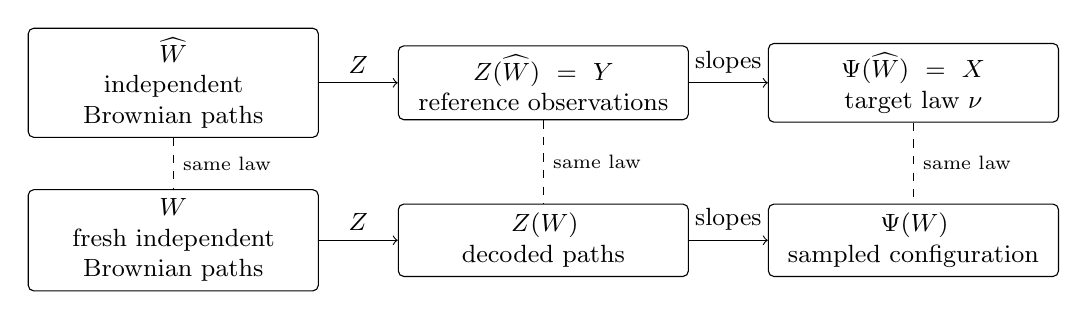
\begin{tikzpicture}[box/.style={draw,rounded corners=2pt,align=center,
  minimum height=0.85cm,text width=3.45cm},font=\small]
\node[box] (a) at (0,0) {$\widehat W$\\independent Brownian paths};
\node[box] (b) at (4.7,0) {$Z(\widehat W)=Y$\\reference observations};
\node[box] (c) at (9.4,0) {$\Psi(\widehat W)=X$\\target law $\nu$};
\node[box] (d) at (0,-2) {$W$\\fresh independent Brownian paths};
\node[box] (e) at (4.7,-2) {$Z(W)$\\decoded paths};
\node[box] (f) at (9.4,-2) {$\Psi(W)$\\sampled configuration};
\draw[->] (a) -- node[above] {$Z$} (b);
\draw[->] (b) -- node[above] {slopes} (c);
\draw[->] (d) -- node[above] {$Z$} (e);
\draw[->] (e) -- node[above] {slopes} (f);
\draw[dashed] (a) -- node[right,font=\scriptsize] {same law} (d);
\draw[dashed] (b) -- node[right,font=\scriptsize] {same law} (e);
\draw[dashed] (c) -- node[right,font=\scriptsize] {same law} (f);
\end{tikzpicture}
\caption{Law transfer in Proposition~\ref{prop:brownian-sampler}.
The upper row is the reference coupling. Deterministic inversion identifies
its middle term pathwise; integer-time slopes recover its right term almost
surely. The lower row uses only independent input paths. Borel measurability
transfers the full joint laws, not only the individual coordinate marginals.}
\label{fig:law-transfer}
\end{figure}

\begin{remark}[The uniformity hypothesis is substantive]
Let $I$ be countably infinite and let $\nu$ assign probability $1/2$ to
each of the all-zero and all-one configurations. For nonempty finite $S$,
all its finite-tilt means are
\[
 b_{i,S}(t,y)=\frac{\exp(a)}{1+\exp(a)},
 \qquad a=\sum_{j\in S}(y_j-t/2).
\]
At $a=0$, the absolute row sum of its field derivatives is $|S|/4$.
Thus no fixed $L$ works along an exhaustion of $I$. The innovation lemma
still applies to this law, but it alone gives no deterministic inverse:
Proposition~\ref{prop:brownian-sampler} uses the uniform response assumption
precisely at that step. Likewise, equivariance of the sampler is asserted
only for relabelings intertwining the chosen drift; arbitrary exhausting
sets need not preserve every symmetry of $\nu$.
\end{remark}

For $\nu=\FUSF_G$, the response bound \eqref{eq:finite-response}
provides the hypothesis of Proposition~\ref{prop:brownian-sampler}
with $L=1/2$.  It remains to obtain the Brownian inputs from the vertex
labels and to verify that the resulting construction is one Borel
rule across graphs.

\section{One Borel graph rule}
\label{sec:implementation}

We implement the preceding construction using only vertex labels and the
distinguished undirected edge. Local finiteness and connectivity imply that
each graph has countably many vertices and edges.

\subsection{From vertex labels to independent edge paths}

\begin{lemma}\label{lem:edge-noise}
There is a Borel equivariant rule assigning a continuous path $w_e$ starting
at zero to each edge of a vertex-labeled graph such that, for every fixed
graph with independent uniform vertex labels, $(w_e)_{e\in E(G)}$ are
independent standard Brownian motions.
\end{lemma}

\begin{proof}
Partition the binary digits of a uniform variable into countably many
infinite subsequences. With a fixed Borel convention at dyadic rationals,
this gives a Borel map from one uniform variable to a countable family of
independent uniforms. At each vertex $v$, use this map to obtain a key $K_v$
and a private sequence $(V_{v,r})_{r\ge1}$, with all these variables independent.
Almost surely the keys are distinct throughout the graph. On this event,
an edge $e=\{u,v\}$ with $K_u<K_v$ selects $V_{u,r}$, where $r$ is the rank
of $v$ among the neighbors of $u$, ordered by key. The rank is finite.
Different edges select different pairs $(u,r)$: edges with different source
vertices use different pools, and edges with the same source vertex have
different other endpoints and hence different ranks. Simplicity is used here.
Conditional on all the keys, the selected variables are distinct coordinates
of an independent uniform family that is independent of those keys. They
therefore have the product uniform law.

For completeness, one uniform can be mapped Borel measurably to a standard
Brownian path. Split it into uniforms and apply the normal quantile to
obtain independent standard normals, using finite defaults at exceptional
quantile inputs. Start at $w(0)=0$ and use some of them as independent increments on the
nonnegative integer grid. On an interval $[a,a+h]$ of a dyadic grid, insert
the midpoint value
\[
 \frac{w(a)+w(a+h)}2+\frac{\sqrt h}{2}\,\xi,
\]
where $\xi$ is a fresh independent standard normal. The two new increments
are jointly Gaussian, have variance $h/2$, and have covariance zero. By
induction, every dyadic grid has independent Gaussian increments of the
appropriate variances.

On $[0,K]$, with $K$ a positive integer, the refinement of mesh $2^{-p}$
uses $K2^p$ new normals. The probability that any has absolute value greater
than $p$ is at most $2K2^p e^{-p^2/2}$, which is summable for $p\ge1$.
The change of linear interpolation at that level is therefore eventually
at most $p2^{-p/2}/2$. These bounds are summable. The interpolations converge
uniformly on every compact interval almost surely. Their limit has continuous
paths and the required dyadic Gaussian laws, hence the Wiener law by
continuity. The event of compact-uniform convergence is Borel: it is the
countable collection of uniform Cauchy conditions on integer intervals.
Each condition can be tested at rational times for these continuous
interpolations. Taking the limit on this event and the zero path otherwise
defines a Borel path-valued map on every input.

Apply this same map to every selected edge uniform. This produces the
required product Wiener law. On a labeling with any repeated keys, assign
the zero path to every edge. A key collision is witnessed in some finite
ball about the distinguished edge, so this exceptional case is Borel and
equivariant. It has probability zero on each fixed countable graph. All
other selections involve only finite neighbor lists and are Borel and
equivariant as well.
\end{proof}

\subsection{Measurability on varying graphs}

The decoder must be one rule on graph space, in addition to being Borel for
each fixed graph. We give the details of this point. On the Borel set of
labelings with distinct keys, vertices in any finite ball can be listed in
increasing key order. Its undirected edges can then be listed lexicographically by
$(\min\{K_u,K_v\},\max\{K_u,K_v\})$. These are finite measurable listings, not a global ordering
of the vertices. Re-distinguishing the graph at any edge selected from such
a list is a Borel operation: each finite neighborhood of that edge can be
read in a sufficiently large finite neighborhood of the original edge.
For example, if the selected edge lies in $H_r(e)$, its radius-$q$
neighborhood is visible in $H_{r+q+1}(e)$. In particular, a Borel edge rule
may be evaluated measurably at the finitely many edges in any such ball.
The evaluated rule may itself depend on the entire graph; measurability
follows by composition with re-distinguishing, not from finite dependence.

For the drift from Section~\ref{sec:response}, every
$b_{e,S_n(e)}(t,y)$ is the limit of a finite weighted-tree ratio on $H_m(e)$
as $m\to\infty$, with $n$ held fixed. The finite ratio uses only finitely
many current fields and the finite graph. The outer limsup in $n$ then
defines $b_e(t,y)$. This exact order of limits makes the formula Borel when
the current fields are supplied by any Borel edge rule jointly measurable
in $t$.

Start with the paths $Z_e^0(t)=w_e(t)$ from Lemma~\ref{lem:edge-noise}.
They are jointly Borel in the labeled graph, the distinguished edge, and
$t$. If the same is true of $Z^k$, the preceding finite listings and drift
formula show that
\[
 (G,U,e,s)\longmapsto b_e(s,Z^k(s))
\]
is Borel and bounded. Its scalar parameter integral over $[0,t]$ is Borel
in $(G,U,e,t)$: on $0\le t\le T$ it is the integral over $[0,T]$ of the
bounded Borel function multiplied by $\1_{\{s\le t\}}$. This is the usual
measurability of integration with respect to a fixed finite measure, proved
first for indicator rectangles and then by bounded approximation. Thus
the next Picard iterate is jointly Borel. The countable limit defining
$Z$, and the integer-time limsup in \eqref{eq:readout}, preserve Borel
measurability.

Every operation commutes with labeled isomorphisms. In particular, the balls
$H_n(e)$ are centered on the unordered endpoints of $e$, and the finite
key order is transported by any labeled isomorphism. Scalar time integration
and the prescribed countable limits preserve this invariance. There is no
distinguished vertex or external enumeration in the construction.

\begin{proof}[Proof of Theorem~\ref{thm:main}]
On labelings with distinct keys, define $\Phi(G,U,e)$ by the readout
\eqref{eq:readout}, using the intrinsic forest drift and the edge paths of
Lemma~\ref{lem:edge-noise}. On the remaining labelings set $\Phi=0$ at every
edge. The preceding argument makes this a single Borel, root-independent,
equivariant rule, defined on all labelings.

Fix a graph $G$. Its key-collision event has probability zero, and the edge
paths have product Wiener law. Lemma~\ref{lem:forest-response} gives the
uniform finite-tilt response bound with $L=1/2$ for $\nu=\FUSF_G$.
Proposition~\ref{prop:brownian-sampler} therefore identifies the joint law
of all the output indicators as $\FUSF_G$. This proves the assertion for
every fixed graph.
\end{proof}

\begin{proof}[Proof of Corollary~\ref{cor:unimodular}]
Place independent uniform labels conditionally on $(G,o)$. The graphwise
conclusion of Theorem~\ref{thm:main}, for the same Borel rule $\Phi$, gives
the desired conditional law. This is an equality of conditional probability
kernels for each graph; it requires no intersection of label-conull sets
over different graphs. Unimodularity imposes no further requirement on the
construction.
\end{proof}

\section{Strongly Rayleigh processes on countable groups}
\label{sec:strongly-rayleigh}

The finite response hypothesis of Proposition~\ref{prop:brownian-sampler}
holds for every strongly Rayleigh law. The fixed-cardinality covariance
identity for trees becomes an inequality for this larger class.
The covariance-row estimate below appears in Alishahi, Barzegar, and
Zamani~\cite[Lemma~2.5 and (1)]{AlishahiBarzegarZamani2023}, following the
nonnegative-row-sum result of Ghosh, Liggett, and
Pemantle~\cite[arXiv version, Lemma~3.2]{GhoshLiggettPemantle2017}.
We give a proof by symmetric homogenization and apply it uniformly after
positive external-field tilts.

\begin{lemma}[Strongly Rayleigh response]\label{lem:sr-response}
Let $F$ be a nonempty finite set and let $\mu$ be a strongly Rayleigh
probability law on $\{0,1\}^F$. For $h\in\R^F$, let
\[
 \mu_h(x)=\frac{\exp(\sum_{j\in F}h_jx_j)\mu(x)}
 {\sum_{z\in\{0,1\}^F}\exp(\sum_{j\in F}h_jz_j)\mu(z)},
 \qquad p_i(h)=\E_{\mu_h}X_i.
\]
For every $i,j\in F$, the derivative identity below holds, and for every
$i\in F$ the row satisfies
\begin{equation}\label{eq:sr-covariance-row}
 \frac{\partial p_i}{\partial h_j}
 =\Cov_{\mu_h}(X_i,X_j),
 \qquad
 \sum_{j\in F}\left|\frac{\partial p_i}{\partial h_j}\right|
 \le 2p_i(h)(1-p_i(h))\le\frac12.
\end{equation}
Consequently
\begin{equation}\label{eq:sr-response}
 |p_i(h)-p_i(h')|\le\frac12\max_{j\in F}|h_j-h'_j|
 \qquad(h,h'\in\R^F).
\end{equation}
\end{lemma}

\begin{proof}
The tilted generating polynomial is
\[
 g_{\mu_h}(z)
 =\frac{g_\mu((e^{h_j}z_j)_{j\in F})}
        {g_\mu((e^{h_j})_{j\in F})}.
\]
The denominator is positive. Positive coordinate scaling preserves
stability, so $\mu_h$ is strongly Rayleigh; see
Borcea, Br\"and\'en, and Liggett~\cite[Section~2.1(iv) and Proposition~3.1(2)]{BorceaBrandenLiggett2009}.
Differentiating the finite partition sum gives the covariance identity in
\eqref{eq:sr-covariance-row}.

Write $n=|F|$ and $\eta=\mu_h$. To recover a constant total count, take a
disjoint set $F'$ of $n$ dummy coordinates. First sample the occupied set
$A\subseteq F$ with law $\eta$; conditional on $A$, occupy a uniformly
chosen subset of $F'$ of size $n-|A|$. The resulting law
$\widetilde\eta$ keeps $\eta$ as its $F$-marginal and has exactly $n$
occupied coordinates in total. Write $\eta(A)$ for the probability of the
occupied set $A$, and let $e_k$ be the elementary symmetric polynomial
of degree $k$ in $w=(w_j)_{j\in F'}$. The generating polynomial of
$\widetilde\eta$, called the symmetric homogenization of $g_\eta$, is
\[
 \widetilde g(z,w)
 =\sum_{A\subseteq F}\eta(A)\prod_{j\in A}z_j\,
       \frac{e_{n-|A|}(w)}{\binom{n}{|A|}}.
\]
The polynomial has nonnegative coefficients, equals one at the
all-one vector, is homogeneous of degree $n$, and specializes to $g_\eta$
when all the $w$ variables equal one. The additional fact that it is stable
is supplied by
\cite[Definition~2.12 and Theorem~4.2]{BorceaBrandenLiggett2009}.
Thus $\widetilde\eta$ is strongly Rayleigh.

Let $C_{jk}=\Cov_{\widetilde\eta}(X_j,X_k)$. The Rayleigh inequality
in~\cite[Theorem~4.1]{BorceaBrandenLiggett2009}, evaluated at the all-one
vector, gives $C_{jk}\le0$ for $j\ne k$. Since the total count is constant,
for $i\in F$ we have
\[
 0=\sum_{j\in F\sqcup F'}C_{ij}
  =C_{ii}+\sum_{j\in F\setminus\{i\}}C_{ij}
            +\sum_{j\in F'}C_{ij}.
\]
The dummy covariances in the last sum are nonpositive. It follows that
\[
 -\sum_{j\in F\setminus\{i\}}C_{ij}
 =C_{ii}+\sum_{j\in F'}C_{ij}\le C_{ii},
 \qquad
 \sum_{j\in F}|C_{ij}|\le2C_{ii}.
\]
The covariances with both indices in $F$ are those of $\eta$, and
$C_{ii}=p_i(h)(1-p_i(h))\le1/4$. This proves
\eqref{eq:sr-covariance-row}, including degenerate coordinates. No
homogeneity or full-support assumption on $\mu$ was used. Integrating the
gradient along the segment from $h$ to $h'$ proves \eqref{eq:sr-response}.
\end{proof}

\begin{proof}[Proof of Theorem~\ref{thm:sr-group}]
Fix a site $i\in\Gamma$ and a finite observed set $S\subseteq\Gamma$.
Let $J=S\cup\{i\}$ and let $\nu_J$ be the marginal of $\nu$ on $J$.
For $t\ge0$ and $y\in\R^\Gamma$, tilt $\nu_J$ by
\[
 \exp\!\left(\sum_{j\in S}(y_j-t/2)x_j\right).
\]
The resulting probability law $\eta_{t,y}$ is an arbitrary positive
external-field tilt of the strongly Rayleigh law $\nu_J$, with zero log
field on $J\setminus S$. Its mean at $i$ is exactly the finite-tilt
function $b_{i,S}(t,y)$ in \eqref{eq:finite-tilt}. Finite differentiation
and Lemma~\ref{lem:sr-response} give
\[
 \frac{\partial b_{i,S}}{\partial y_j}(t,y)
 =\Cov_{\eta_{t,y}}(X_i,X_j)\quad(j\in S),
 \qquad
 \sum_{j\in S}\left|\frac{\partial b_{i,S}}{\partial y_j}(t,y)\right|
 \le\sum_{j\in J}|\Cov_{\eta_{t,y}}(X_i,X_j)|\le\frac12.
\]
Integrating along a segment of fields yields
\begin{equation}\label{eq:sr-finite-tilt}
 |b_{i,S}(t,y)-b_{i,S}(t,y')|
 \le\frac12\max_{j\in S}|y_j-y'_j|.
\end{equation}
For $S=\varnothing$, the finite-tilt function is constant and the same
statement holds with the empty maximum defined to be zero. The bound is
uniform in $i,S,t$ and in all finite field values. It uses the actual
finite marginal of $\nu$, with no infinite external-field tilt or
finite-volume approximation.

Choose finite sets $F_n\subseteq\Gamma$ increasing to $\Gamma$, with the
identity in every $F_n$, and put
\[
 S_n(h)=hF_n,\qquad h\in\Gamma.
\]
These are finite exhaustions at every site, and
$S_n(gh)=gS_n(h)$ for all $g,h\in\Gamma$. This requires neither finite
generation nor amenability; for a finite group one may take $F_n=\Gamma$.
Invariance of $\nu$ gives the exact finite-tilt identity
\begin{equation}\label{eq:sr-tilt-equivariance}
 b_{gh,gS}(t,\tau_g y)=b_{h,S}(t,y)
\end{equation}
for every $g,h,t,y$ and finite $S$. Indeed, in the numerator and denominator
of \eqref{eq:finite-tilt}, substitute $x=\tau_g z$. Then
$x_{gh}=z_h$, $(\tau_g y)_{gs}=y_s$, and $x_{gs}=z_s$, while the law of
$z$ is again $\nu$. All sums are finite, so the identity holds pointwise
even when the complete field is unbounded.

Define the limsup drift using these $S_n(h)$. Equations
\eqref{eq:sr-tilt-equivariance} and $S_n(gh)=gS_n(h)$ give
\[
 b_{gh}(t,\tau_g y)
 =\limsup_n b_{gh,S_n(gh)}(t,\tau_g y)
 =\limsup_n b_{h,S_n(h)}(t,y)=b_h(t,y).
\]
Thus the drift is equivariant under every regular left translation on its
entire domain. The uniform bound \eqref{eq:sr-finite-tilt} supplies the
hypothesis of Proposition~\ref{prop:brownian-sampler} with $L=1/2$.
That proposition gives a Borel map $\Psi$ from the product continuous-path
space to $\{0,1\}^{\Gamma}$, sending independent standard Brownian paths
to $\nu$ and commuting with every $\tau_g$ on every input.

The proof of Lemma~\ref{lem:edge-noise} constructs an everywhere-defined
Borel map from one uniform variable to a standard Brownian path, with fixed
defaults on its exceptional inputs. Applying this map coordinatewise
sends independent uniform labels on $\Gamma$ to independent Brownian paths
and commutes with all translations. Its composition with $\Psi$ is the
required map $\Phi_\nu$.
\end{proof}

The sets $F_n$ above need not be F\o lner sets. Their translated form is
available because the action is regular. For an arbitrary action on another
countable set, equivariant finite exhaustions are not automatic, and no
such extension is asserted here.

\begin{proof}[Proof of Corollary~\ref{cor:dpp-group}]
For a countable discrete set, every self-adjoint positive contraction
defines a determinantal probability law; see Lyons~\cite[Section~8]{Lyons2003}.
For a finite $J\subseteq\Gamma$, let $K_J$ be the compression of $K$ to
$\ell^2(J)$. It is a Hermitian positive contraction. For every $A\subseteq J$,
the inclusion probability of $A$ under the $J$-marginal is
\[
 \P(A\subseteq X)=\det K_{A,A}=\det (K_J)_{A,A}.
\]
These inclusion probabilities determine the finite binary law by
inclusion--exclusion. Hence that marginal is the determinantal law with
kernel $K_J$, and it is strongly Rayleigh by
\cite[Proposition~3.5]{BorceaBrandenLiggett2009}. This covers complex
Hermitian, singular, and projection kernels; no trace-class condition on
the operator on $\ell^2(\Gamma)$ is needed. Theorem~\ref{thm:sr-group}
now applies whenever the determinantal law is translation invariant.

If $K$ commutes with the left regular representation, its matrix entries
satisfy $K_{gh,gk}=K_{h,k}$. All finite inclusion determinants are then
translation invariant. Inclusion--exclusion and the uniqueness of a
countable law from its cylinder probabilities give invariance of the
determinantal law, proving the final assertion.
\end{proof}

\bibliographystyle{plain}
\bibliography{references}
\end{document}
